\documentclass[tikz,border=12pt]{standalone}
\usepackage{tikz}
\usetikzlibrary{shapes.misc}
\begin{document}
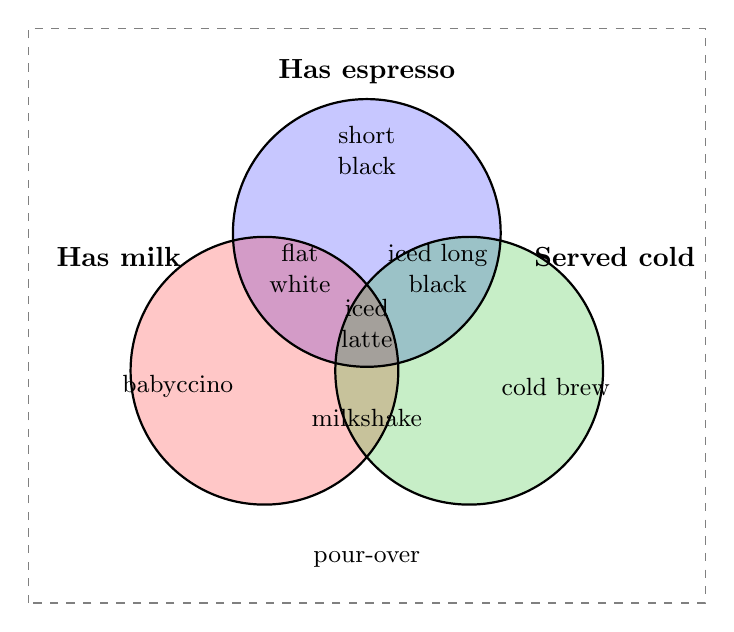
\begin{tikzpicture}
  \def\r{1.7}
  \coordinate (E) at (0,1);
  \coordinate (M) at (-1.3,-0.75);
  \coordinate (C) at (1.3,-0.75);

  % Universe
  \draw[dashed,gray] (-4.3,-3.7) rectangle (4.3,3.6);

  % Fills
  \begin{scope}[fill opacity=0.22]
    \fill[blue] (E) circle (\r);
    \fill[red]  (M) circle (\r);
    \fill[green!70!black] (C) circle (\r);
  \end{scope}

  % Outlines
  \draw[thick] (E) circle (\r);
  \draw[thick] (M) circle (\r);
  \draw[thick] (C) circle (\r);

  % Circle labels
  \node[font=\bfseries] at (0,3.05) {Has espresso};
  \node[font=\bfseries] at (-3.15,0.7) {Has milk};
  \node[font=\bfseries] at (3.15,0.7) {Served cold};

  % Region labels
  \node[align=center,font=\small] at (0,2.05) {short\\black};
  \node[align=center,font=\small] at (-0.85,0.55) {flat\\white};
  \node[align=center,font=\small] at (0.9,0.55) {iced long\\black};
  \node[align=center,font=\small] at (0,-0.15) {iced\\latte};
  \node[align=center,font=\small] at (-2.4,-0.95) {babyccino};
  \node[align=center,font=\small] at (2.4,-0.95) {cold brew};
  \node[align=center,font=\small] at (0,-1.35) {milkshake};
  \node[align=center,font=\small] at (0,-3.15) {pour-over};
\end{tikzpicture}
\end{document}
